%%%%%%%%%%%%%%%%%%%%%%%%%%%%%%%%%%%%%%%%%
% Tecnológico de Costa Rica/Instructivo de Laboratorio de Instrumentación I
% LaTeX Template
% Version 3.1 (25/3/14)
%
% This template has been downloaded from:
% http://www.LaTeXTemplates.com
%
% Original author:
% Linux and Unix Users Group at Virginia Tech Wiki 
% (https://vtluug.org/wiki/Example_LaTeX_chem_lab_report)
%
% License:
% CC BY-NC-SA 3.0 (http://creativecommons.org/licenses/by-nc-sa/3.0/)
%
%%%%%%%%%%%%%%%%%%%%%%%%%%%%%%%%%%%%%%%%%

%----------------------------------------------------------------------------------------
%	PACKAGES AND DOCUMENT CONFIGURATIONS
%----------------------------------------------------------------------------------------

\documentclass[12pt,letterpaper]{report}
\usepackage{amsmath}
\usepackage{amssymb}
\usepackage{siunitx}
\usepackage{float}
\usepackage{tikz}
\def\checkmark{\tikz\fill[scale=0.4](0,.35) -- (.25,0) -- (1,.7) -- (.25,.15) -- cycle;} 
\usepackage{url}
\usepackage[siunitx,american,RPvoltages]{circuitikz}
\ctikzset{capacitors/scale=0.7}
\ctikzset{diodes/scale=0.7}
\usepackage{tabularx}
\newcolumntype{C}{>{\centering\arraybackslash}X}
\renewcommand\tabularxcolumn[1]{m{#1}}% for vertical centering text in X column
\usepackage{tabu}
\usepackage[spanish,es-tabla,activeacute]{babel}
\usepackage{babelbib}
\usepackage{booktabs}
\usepackage{pgfplots}
\usepackage{hyperref}
\hypersetup{colorlinks = true,
            linkcolor = black,
            urlcolor  = blue,
            citecolor = blue,
            anchorcolor = blue}
\usepgfplotslibrary{units, fillbetween} 
\pgfplotsset{compat=1.16}
\usepackage{bm}
\usetikzlibrary{arrows, arrows.meta, shapes, 3d, perspective, positioning}
\renewcommand{\sin}{\sen} %change from sin to sen
\usepackage{bohr}
\setbohr{distribution-method = quantum,insert-missing = true}
\usepackage{elements}
\usepackage{verbatim}
\usetikzlibrary{mindmap,trees,backgrounds}
 
\definecolor{color_mate}{RGB}{255,255,128}
\definecolor{color_plas}{RGB}{255,128,255}
\definecolor{color_text}{RGB}{128,255,255}
\definecolor{color_petr}{RGB}{255,192,192}
\definecolor{color_made}{RGB}{192,255,192}
\definecolor{color_meta}{RGB}{192,192,255}
\usepackage[edges]{forest}
\usepackage{etoolbox}
\usepackage{schemata}
\newcommand\diagram[2]{\schema{\schemabox{#1}}{\schemabox{#2}}}
\usepackage{listofitems}
\usepackage{csvsimple}
\usepackage{geometry} 
\geometry{left=18mm,right=18mm,top=21mm,bottom=21mm,headheight=15pt}

\setlength\parindent{0pt} % Removes all indentation from paragraphs

\renewcommand{\labelenumi}{\alph{enumi}.} % Make numbering in the enumerate environment by letter rather than number (e.g. section 6)
\usepackage{fancyhdr}
\pagestyle{fancy}

%----------------------------------------------------------------------------------------
\lhead{Instructivo de Prácticas - Instrumentación II}
\rhead{\begin{picture}(0,0) \put(-60,0){
\includegraphics[width=20mm]{fig/comunes/logo.png}} \end{picture}}
\newcommand{\obj}{Objetivos}
\newcommand{\mat}{Materiales y equipo}
\newcommand{\pro}{Procedimiento}
\newcommand{\capacidad}{Al finalizar este laboratorio el estudiante estará en capacidad de:}
\newcommand{\antesde}{Antes de empezar el laboratorio presente el siguiente cuestionario lleno.}
%----------------------------------------------------------------------------------------
%	DOCUMENT INFORMATION
%----------------------------------------------------------------------------------------


\addto\captionsspanish{\renewcommand{\chaptername}{Práctica}}
\addto\captionsspanish{\renewcommand{\tablename}{Tabla}}
\begin{document}


\begin{titlepage}

\begin{center}
\vspace*{1in}
\begin{figure}[htb]
\begin{center}

\includegraphics[width=11cm]{fig/comunes/logo.png}
\end{center}
\end{figure}
\vspace*{0.4in}
\begin{Huge}
Escuela de Física\\
\vspace*{0.15in}
Ingeniería Física\\
\vspace*{0.8in}
\end{Huge}
\vspace*{0.2in}
\begin{Large}
\textbf{Instructivo de Prácticas} \\
\end{Large}
\vspace*{0.3in}
\begin{large}
Instrumentación II\\
\end{large}
\vspace*{2.5in}
\begin{Large}
\textbf{\today}\\
Versión: 0.2\\
\end{Large}
\rule{80mm}{0.1mm}\\
\vspace*{0.1in}
\begin{large}
Realizado por: Juan J. Rojas\\
\end{large}
\end{center}

\end{titlepage}

\tableofcontents

\chapter{Implementación de un instrumento virtual básico}
\section{\obj}
\capacidad
\begin{itemize}
\item Implementar un instrumento virtual básico.
\item Implementar una interfaz de usuario básica.
\item Utilizar un DAQ para medir corriente y voltaje.
\end{itemize}

\section{\mat}
\textbf{A suministrar por la Escuela:}
\begin{itemize}
\item 1 dispositivo de adquisición de datos NI myDAQ

\end{itemize}
\textbf{A suministrar por el estudiante:}
\begin{itemize}
\item 1 breadboard
\item 1 potenciometro de \SI{10}{\kilo\ohm}
\item 1 resistor de \SI{220}{\ohm} y \SI{0.25}{\watt}
\item Cables de interconexión (jumpers) macho-macho
\end{itemize}


\section{\pro}
\begin{enumerate}
\item Realice las conexiones del circuito tal y como se indica en la Figura \ref{fig:L1F1}.
\begin{figure}[H]
    \centering
    \begin{circuitikz} 
        \draw
        (5.5,3) node[ground]{}
            to[V] 
        (5.5,6) node[above]{$+$\SI{15}{\volt}} 
            --
        (3,6)
        	to[american potentiometer,n=mypot, l_=0$\sim$\SI{10}{\kilo\ohm},i=$i$]
        (3,3) 
        %(mypot.wiper) to[short,-o] ++(2,0)
        (3,3)
            to[R, l_=\SI{200}{\ohm}, v^=$v$]
        (3,0)
            --
        (3,-0.5)
            --
        (5.5,-0.5) node[ground]{}node[above]{AGND}
        ;
        \draw 
        (5.5,1.5) node[op amp, noinv input up](opamp){AI0}
        (opamp.+) --++ (-0.5,0) --++ (0,0.7) to[short,-*]++ (-0.8,0)
        (opamp.-) --++ (-0.5,0) --++ (0,-0.7) to[short,-*]++ (-0.8,0)
        ;
        \draw[dashed,blue]
        (4,8) -- (7,8)node[midway, below]{myDAQ} -- (7,-1.5) -- (4,-1.5) -- (4,8);
    \end{circuitikz}
    \caption{Medición de corriente y voltaje en un circuito.}
    \label{fig:L1F1}
\end{figure}
\item Cree un instrumento virtual (\emph{.vi}) que realice lo siguiente:
    \begin{itemize}
        \item Leer en un While 100 muestras del valor de AI0 durante \SI{100}{\milli\second} y las promedie
        \item Calcular el valor promedio de las muestras obtenidas $v$ cada \SI{100}{\milli\second} y lo muestre en un gráfica en el panel frontal
        \item Calcular el valor promedio de las muestras obtenidas $i$ cada \SI{100}{\milli\second} y lo muestre en un gráfica en el panel frontal
        \item Iniciar la gráfica vacía. 
        \item Detener la toma de datos después de \SI{10}{\second}
    \end{itemize}
\item Una vez realizado el instrumento virtual córralo, modifique de forma aleatoria el valor del potenciometro y guarde los datos de las gráficas como archivos \emph{.csv}.
\item Incluya en su informe lo siguiente:
    \begin{itemize}
        \item Una captura de pantalla del diagrama de bloques
        \item Una captura de pantalla del panel frontal
        \item Una gráfica de $i$ realizada a partir del archivo \emph{.csv}, usando Python. Incluya los títulos de los ejes de forma adecuada. 
        \item Una gráfica de $v$ realizada a partir del archivo \emph{.csv}, usando Python. Incluya los títulos de los ejes de forma adecuada. 
    \end{itemize}
\end{enumerate}

\chapter{Estructuras de datos}
\section{\obj}
\capacidad
\begin{itemize}
\item Comprender las diferentes estructuras de datos.
\item Realizar mediciones en mas de un canal al mismo tiempo.
\end{itemize}

\section{\mat}
\textbf{A suministrar por la Escuela:}
\begin{itemize}
\item 1 dispositivo de adquisición de datos NI myDAQ
\item 1 interruptor rotativo de 16 posiciones 

\end{itemize}
\textbf{A suministrar por el estudiante:}
\begin{itemize}
\item 1 breadboard
\item Cables de interconexión (jumpers) macho-macho
\end{itemize}

\section{\pro}
\begin{enumerate}
\item Realice las conexiones del circuito tal y como se indica en la Figura \ref{fig:L2F1}.

\item Cree un instrumento virtual (\emph{.vi}) que realice lo siguiente:
    \begin{itemize}
        \item Leer en un While 1 muestra del valor de las entradas DIO0, DIO1, DIO2 y DIO3 cada \SI{500}{\milli\second} y mostrarla como una matriz de booleano
        \item Convertir el valor binario obtenido en un numero entero y mostrarlo en el panel frontal
        \item Dividir el numero entero obtenido entre el valor máximo (15) y mostrar el valor en un ``Slide''
        \item Convertir el numero entero obtenido en una cadena hexadecimal
        \item Mostrar un mensaje en el panel frontal que diga ``El selector está en XX'' donde XX es la cadena hexadecimal obtenida. 
        \item Guardar la cadena hexadecimal obtenida en una matriz cada vez que exista un cambio de valor
    \end{itemize}
\begin{figure}[H]
    \tikzset{demux/.style={muxdemux, muxdemux def={Lh=4, Rh=3, NL=4, NB=0, NR=1, w=2}}}
    \tikzset{switch16/.style={muxdemux, muxdemux def={Lh=3, Rh=3, NL=3, NB=0, NR=3, w=2}}}
    \centering
    \begin{circuitikz} 
        \draw (0,0) node[demux] (m){\rotatebox{90}{\small multiplex}}
        ;
        \foreach \i in {0,...,3}
        {
            \pgfmathtruncatemacro{\pin}{\i + 1}
            \draw (m.blpin \pin) node[above left]{\small DI0\i};
        }
        \draw (-4,2) node[switch16,rotate=90] (s){\rotatebox{-90}{\small switch}}
        (s.brpin 3) node[above right]{\small 1}
        (s.brpin 2) node[above right]{\small C}
        (s.brpin 1) node[above right]{\small 4}
        (s.blpin 3) node[below right]{\small 8}
        (s.blpin 2) node[below right]{\small C}
        (s.blpin 1) node[below right]{\small 2}
        ;
        \draw
        (0,2) node[ground]{}
            to[V] 
        (0,4) node[above]{\SI{5}{\volt}} 
            --
        (-3,4)
            -|
        (s.brpin 2)
        ;
        \draw[red]
        (m.blpin 1) --++ (-2,0) --++ (0,2.5) -| (s.brpin 3)
        ;
        \draw[blue]
        (m.blpin 2) -| (s.blpin 1)
        ;
        \draw[orange]
        (m.blpin 3) --++ (-5,0) --++ (0,3.5) -| (s.brpin 1)
        ;
        \draw[brown]
        (m.blpin 4) -| (s.blpin 3)
        ;
        \draw[dashed,blue]
        (-1.6,6) -- (1,6)node[midway, below]{myDAQ} -- (1,-1.5) -- (-1.6,-1.5) -- cycle;
    \end{circuitikz}
    \caption{Lectura de estados de un interruptor rotativo de 16 posiciones.}
    \label{fig:L2F1}
\end{figure}
\item Una vez realizado el instrumento virtual, córralo, realice al menos 10 cambios y guarde los datos de la matriz de cadenas hexadecimales como un archivo de Excel.
\item Incluya en su informe lo siguiente:
    \begin{itemize}
        \item Una captura de pantalla del diagrama de bloques
        \item Una captura de pantalla del panel frontal
        \item Una tabla con los valores de las cadenas hexadecimales obtenidas.  
    \end{itemize}
\end{enumerate}

Detalle del interruptor rotativo:
\begin{center}
    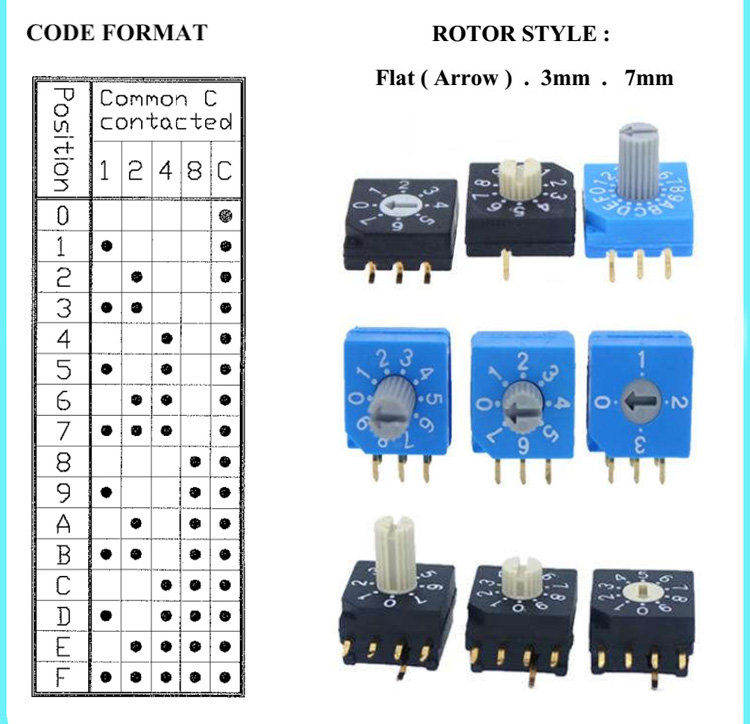
\includegraphics[width=0.3\textwidth]{fig/rotary_switch.jpg}
\end{center}

\chapter{Estructuras de ejecución}
\section{\obj}
\capacidad
\begin{itemize}
\item Comprender las diferentes estructuras de ejecución.
\item Realizar mediciones detenidas programáticamente.
\end{itemize}

\section{\mat}
\textbf{A suministrar por la Escuela:}
\begin{itemize}
\item 1 dispositivo de adquisición de datos NI myDAQ
\item 1 termistor TDC310 de \SI{10}{\kilo\ohm} 
\item 1 resistor de \SI{10}{\kilo\ohm}
\item 1 capacitor de \SI{0.1}{\micro\farad}

\end{itemize}
\textbf{A suministrar por el estudiante:}
\begin{itemize}
\item 1 breadboard
\item Cables de interconexión (jumpers) macho-macho
\end{itemize}


\section{\pro}
\begin{enumerate}
\item Realice las conexiones del circuito tal y como se indica en la Figura \ref{fig:L1F1}.
\item Cree un instrumento virtual (\emph{.vi}) que realice lo siguiente:
    \begin{itemize}
        \item Leer en una estructura temporizada 500 muestras del valor de $v$ cada \SI{500}{\milli\second}, sacar el promedio de las muestras y mostrarlo en un indicador.
        \item Calcular el valor de la resistencia del termistor usando la siguiente ecuación y graficarla en tiempo real en el panel frontal.
        \begin{equation*}
            R_T = \dfrac{R}{\frac{5}{v} - 1}
        \end{equation*}
        \item Calcular el valor de la temperatura utilizando la siguiente ecuación y graficarlo en tiempo real en el panel frontal.
        \begin{equation*}
            T = \dfrac{\beta T_0}{\beta + T_0\ln{\left(\frac{R_T}{R_0}\right)}}
        \end{equation*}
        donde $\beta = 4100$, $T_0 = \SI{298.15}{\kelvin}$ y $R_0 = \SI{10}{\kilo\ohm}$
        \item Guardar los datos tomados en un archivo separado por comas (\emph{.csv}) en \emph{tiempo real}, de forma que la primera columna sea el tiempo y la segunda el valor de la resitencia del termistor y la tercera la temperatura.
        \item Generar un mensaje de alarma que indique cuando la temperatura sobrepasó los \SI{50}{\degreeCelsius}
        \item Detener la ejecución luego de \SI{60}{\second}.
    \end{itemize}
\begin{figure}[H]
    \centering
    \begin{circuitikz} 
        \draw
        (5.5,3) node[ground]{}
            to[V] 
        (5.5,5) node[above]{\SI{5}{\volt}} 
            --
        (3,5)
        	to[short]
        (3,3) 
            to[sR, l_=$R_T$, v^=$v$]
        (3,0)
            to[R, l_=$R$]
        (3,-3)
            --
        (5.5,-3) node[ground]{}node[above]{DGND}
        (3,0)
            to[short]
        (1.5,0)
            to[C, l_=$C$]
        (1.5,-3)
            to[short]
        (3,-3)
        ;
        \draw 
        (5.5,1.5) node[op amp, noinv input up](opamp){AI0}
        (opamp.+) --++ (-0.5,0) --++ (0,0.7) to[short,-*]++ (-0.8,0)
        (opamp.-) --++ (-0.5,0) --++ (0,-0.7) to[short,-*]++ (-0.8,0)
        ;
        \draw[dashed,blue]
        (4,7) -- (7,7)node[midway, below]{myDAQ} -- (7,-4) -- (4,-4) -- (4,7);
        \node at (-3,4) {$R_T=\SI{10}{\kilo\ohm}@\SI{298.15}{\kelvin}$}; 
        \node at (-3,3.5) {$R=\SI{10}{\kilo\ohm}$}; 
        \node at (-3,3) {$C=\SI{0.1}{\micro\farad}$}; 
    \end{circuitikz}
    \caption{Medición de caída de voltaje en un termistor.}
    \label{fig:L3F1}
\end{figure}

\item Incluya en su informe lo siguiente:
    \begin{itemize}
        \item Una captura de pantalla del diagrama de bloques
        \item Una captura de pantalla del panel frontal
        \item Una gráfica de $R_T$ realizada a partir del archivo \emph{.csv}, usando Python. Incluya los títulos de los ejes de forma adecuada. 
        \item Una gráfica de $T$ realizada a partir del archivo \emph{.csv}, usando Python. Incluya los títulos de los ejes de forma adecuada. 
    \end{itemize}
    
\end{enumerate}

\chapter{Manejo de archivos y protocolos de comunicación serial}
\section{\obj}
\capacidad
\begin{itemize}
\item Guardar mediciones en archivos para uso posterior.
\item Implementar diferentes protocolos de comunicación serial. 
\end{itemize}

\section{\mat}
\textbf{A suministrar por la Escuela:}
\begin{itemize}
\item 1 dispositivo de adquisición de datos NI myRIO
\item 1 adaptador para breadboard DIGILENT
\item 1 modulo lector de termocupla K basado en el integrado \href{https://datasheets.maximintegrated.com/en/ds/MAX31855.pdf}{MAX31855}
\item 1 display de 7 segmentos y 4 digitos, \href{https://github.com/sparkfun/Serial7SegmentDisplay/wiki/Serial-7-Segment-Display-Datasheet}{COM-11441}

\end{itemize}
\textbf{A suministrar por el estudiante:}
\begin{itemize}
\item Cables de interconexión (jumpers) macho-macho
\end{itemize}


\section{\pro}
\begin{enumerate}
\item Realice las conexiones del circuito tal y como se indica en la Figura \ref{fig:L4F1}.
\item Cree un instrumento virtual (\emph{.vi}) que realice lo siguiente:
    \begin{itemize}
        \item Leer en en un estructura temporizada el valor de la temperatura de la unión fría y la unión caliente ($T$) cada \SI{1000}{\milli\second}, y mostrarlo en un indicador.
        \item Enviar el valor de unión caliente al display de 7 segmentos cada \SI{1000}{\milli\second}.
        \item Guardar los datos tomados en un archivo separado por comas (\emph{.csv}) en \emph{tiempo real}, de forma que la primera columna sea el tiempo y la segunda el valor de la temperatura en la unión caliente y la tercera la temperatura en la unión fría.
        \item Generar un mensaje de alarma que indique cuando la temperatura sobrepasó los \SI{35}{\degreeCelsius}
        \item Detener la ejecución luego de \SI{60}{\second}.
    \end{itemize}
\begin{figure}[H]
    \tikzset{demux/.style={muxdemux, muxdemux def={Lh=4, Rh=3, NL=3, NB=0, NR=1, w=2}}}
    \tikzset{MAX31855/.style={muxdemux, muxdemux def={Lh=5, Rh=5, NL=0, NB=0, NR=6, w=2}}}
    \centering
    \begin{circuitikz} 
    \readlist*\myinputs{06, 11, 05}
        \draw (0,0) node[demux] (m){\rotatebox{90}{\small multiplex}}
        ;
        \foreach \i in {1,...,3}
        {
            
            \pgfmathtruncatemacro{\pin}{\i}
            \draw (m.blpin \pin) node[above left]{\small DI0 \myinputs[\i]};
        }
        \draw (-5,-3) node[MAX31855,rotate=90] (s){\rotatebox{-90}{\small MAX31855}}
        (s.brpin 1) node[above right,rotate=90]{\scriptsize Vin}
        (s.brpin 2) node[above right,rotate=90]{\scriptsize 3V0 / VCC}
        (s.brpin 3) node[above right,rotate=90]{\scriptsize GND}
        (s.brpin 4) node[above right,rotate=90]{\scriptsize DO / SO}
        (s.brpin 5) node[above right,rotate=90]{\scriptsize CS / CS}
        (s.brpin 6) node[above right,rotate=90]{\scriptsize CLK / SCK}
        ;
        \draw
        (0,2) node[ground]{}
            to[V] 
        (0,4) node[above,xshift=-11mm]{+3.3V} 
            --
        (-0.8,4)
        (0,2) node[above,xshift=-11mm]{GND} 
            --
        (-0.8,2)
        ;
        \draw[blue]
        (-0.8,4)
            -|
        (s.brpin 2)
        ;
        \draw[green]
        (-0.8,2)
            -|
        (s.brpin 3)
        ;
        \draw[red]
        (m.blpin 1) --++ (-2,0) -| (s.brpin 4)
        ;
        \draw[yellow]
        (m.blpin 2) --++ (-2,0) -| (s.brpin 5)
        ;
        \draw[brown]
        (m.blpin 3) --++ (-2,0) -| (s.brpin 6)
        ;
        % \draw[blue]
        % (m.blpin 2) -| (s.blpin 1)
        % ;
        \draw[dashed,blue]
        (-1.9,6) -- (1,6)node[midway, below]{myRIO} -- (1,-1.5) -- (-1.9,-1.5) -- cycle;
    \end{circuitikz}
    \caption{Conexión de módulo de lectura de termopar basado en MAX31855.}
    \label{fig:L4F1}
\end{figure}

\item Incluya en su informe lo siguiente:
    \begin{itemize}
        \item Una captura de pantalla del diagrama de bloques
        \item Una captura de pantalla del panel frontal
        \item Una gráfica de $T$ realizada a partir del archivo \emph{.csv}, usando Python. Incluya los títulos de los ejes de forma adecuada. 
    \end{itemize}
    
\end{enumerate}

\chapter{Máquinas de estados}
\section{\obj}
\capacidad
\begin{itemize}
\item Crear máquinas de estados para automatizar procesos de medición.
\end{itemize}

\section{\mat}
\textbf{A suministrar por la Escuela:}
\begin{itemize}
\item 1 dispositivo de adquisición de datos NI myDAQ
\item 1 termistor TDC310 de \SI{10}{\kilo\ohm} 
\item 1 resistor de \SI{10}{\kilo\ohm}
\item 1 capacitor de \SI{0.1}{\micro\farad}

\end{itemize}
\textbf{A suministrar por el estudiante:}
\begin{itemize}
\item 1 breadboard
\item Cables de interconexión (jumpers) macho-macho
\end{itemize}

\section{\pro}
\begin{enumerate}
\item Realice las conexiones del circuito tal y como se indica en la Figura \ref{fig:L3F1}.
\item Cree un instrumento virtual (\emph{.vi}) que realice lo siguiente:
    \begin{itemize}
        \item Crear una máquina de estados que tenga cuatro estados:
            \begin{itemize}
                \item \emph{stand-by}: espera que se presione un botón y pasa al estado \emph{medición}
                \item \emph{medición}: realiza una medición por segundo por $X$\si{\second} y luego pasa al estado de \emph{espera}
                \item \emph{espera}: espera $Z$\si{\second} y continua al estado de medición a menos que una cantidad de tomas de datos mayor a $Y$ haya sido realizada, en ese caso continua al estado  \emph{fin}
                \item \emph{fin}: termina la ejecución del instrumento virtual.
            \end{itemize}
        \item Guardar los datos tomados en cada estado \emph{medición} en un archivo separado por comas (\emph{.csv}) en \emph{tiempo real}, de forma que la primera columna sea el tiempo y la segunda el valor de la temperatura. El archivo debe cambiar de nombre para cada estado \emph{medición}. 
    \end{itemize}
\item Usando Python realice lo siguiente:
\begin{itemize}
    \item Crear una máquina de estados que tenga cinco estados definidos como:
        \begin{itemize}
            \item \emph{stand-by}: estado que espera que se presione el botón, pasa a estado \emph{hello}
            \item \emph{hello}: estado que concatena letra por letra de la palabra "hello" en un string que inicialmente esta vació, debe aparecer una nueva letra cada segundo, al finalizar la palabra pasa a estado \emph{space}
            \item \emph{space}: estado que concatena un espacio vacío al string y espera por 5 segundos, pasa al estado \emph{world}
            \item \emph{world}: estado que concatena letra por letra la palabra "world" en el string, al finalizar la palabra pasa a estado \emph{end}
            \item \emph{end}: estado que termina la ejecución del programa.
        \end{itemize}
    \item Mostrar como avanza la concatenación del string
    \item Mostrar como avanza el tiempo en segundos en cada estado
\end{itemize}
\item Incluya en su informe lo siguiente:
    \begin{itemize}
        \item Una captura de pantalla de cada estado de la máquina 
        \item Una captura de pantalla del panel frontal
        \item Una familia de gráficas de $T$ que incluya todos los datos de los archivos (\emph{.csv}) realizada a partir de los archivos \emph{.csv}, usando Python. Incluya los títulos de los ejes de forma adecuada. 
        \item El archivo \emph{.py} en el que desarrolló la máquina de estados
    \end{itemize}

\end{enumerate}

\chapter{Instrumentos virtuales modulares}
\section{\obj}
\capacidad
\begin{itemize}
\item Crear instrumentos virtuales modulares para simplificar la creación, mantenimiento, documentación y automatización de los procesos de medición.
\end{itemize}

\section{\mat}
\textbf{A suministrar por la Escuela:}
\begin{itemize}
\item 1 dispositivo de adquisición de datos NI myDAQ
\item 1 termistor TDC310 de \SI{10}{\kilo\ohm} 
\item 1 resistor de \SI{10}{\kilo\ohm}
\item 1 capacitor de \SI{0.1}{\micro\farad}

\end{itemize}
\textbf{A suministrar por el estudiante:}
\begin{itemize}
\item 1 breadboard
\item Cables de interconexión (jumpers) macho-macho
\end{itemize}

\section{\pro}
\begin{enumerate}
\item Realice las conexiones del circuito tal y como se indica en la Figura \ref{fig:L3F1}.
\item Cree un instrumento virtual (\emph{.vi}) y realice lo siguiente:
    \begin{itemize}
        \item A partir de la máquina de estados creada en la Práctica 5, cree tres módulos:
            \begin{itemize}
                \item Un módulo que se encargue de la medición de temperatura, una de sus salidas debe ser un arreglo con las mediciones realizadas.  
                \item Un módulo que se encargue de crear los archivos (\emph{.csv}) y guardar los datos en ellos. 
                \item Un módulo que incluya la maquina de estados completa e internamente contenga los dos módulos anteriores.
                \item Un módulo que configure la adquisición de datos.
            \end{itemize}
    \end{itemize}

\item Incluya en su informe lo siguiente:
    \begin{itemize}
        \item Una captura de pantalla de cada módulo 
        \item Una captura de pantalla del panel frontal
    \end{itemize}
    
\end{enumerate}

%	BIBLIOGRAPHY
%----------------------------------------------------------------------------------------

% \bibliographystyle{ieeetr}

% \bibliography{referencias}

%----------------------------------------------------------------------------------------


\end{document}